\section{Fonctionnement des Protocoles Wi-Fi}
\label{sec:protocoles}

La sécurité des réseaux Wi-Fi repose sur une succession de mécanismes cryptographiques introduits progressivement pour corriger les vulnérabilités de leurs prédécesseurs. Depuis \acrshort{wep} en 1997 jusqu'à \acrshort{wpa3} en 2018, chaque protocole a apporté des évolutions majeures : nouveaux algorithmes, nouveaux principes cryptographiques, mécanismes d'intégrité plus robustes, protection des trames de gestion, et résistance aux attaques hors ligne. Cette section propose une analyse approfondie de ces mécanismes, de leurs logiques internes, de leurs limites, ainsi que des structures de trames qu'ils manipulent.

\subsection{Principe général du Wi-Fi}

Le Wi-Fi, ou norme IEEE 802.11, désigne un ensemble de standards pour les réseaux locaux sans fil (WLAN) permettant la transmission de données numériques par ondes radio (principalement 2,4 GHz, 5 GHz et 6 GHz). Développé à partir des années 1990 par le comité IEEE 802.11 pour répondre à la demande croissante de connectivité mobile sans câblage Ethernet, le premier standard a été publié en 1997, révolutionnant l'accès aux données en éliminant les contraintes physiques des réseaux filaires.

Aujourd'hui, le Wi-Fi est omniprésent : points d'accès publics (cafés, aéroports, transports), entreprises, foyers. Avec Wi-Fi 7 (802.11be, 2024) et au-delà, il supporte des débits supérieur à 46 Gbit/s\cite{WiFi7pou99:online}.

\subsection*{Définitions générales Wi-Fi}

Avant d’aborder en détail le fonctionnement des différents protocoles de sécurité, il est utile de préciser brièvement certains termes fondamentaux du Wi-Fi. Le \textbf{\acrfull{ssid}} correspond au nom d’un réseau et permet aux dispositifs de l’identifier lors de la phase de découverte. Le \textbf{\acrfull{bssid}}, quant à lui, désigne l’adresse MAC unique du point d’accès assurant la diffusion du réseau. Le terme \textbf{\acrfull{ap}} désigne ce même point d’accès, tandis que la \textbf{\acrfull{sta}} représente tout client Wi-Fi, qu’il s’agisse d’un ordinateur, d’un smartphone ou d’un objet connecté. La figure \ref{fig:ap_sta_ssid_bssid} illustre les interactions entre les différents appareils.

\begin{figure}[H]
\centering
\begin{tikzpicture}[>=latex, node distance=3cm]

% AP au centre
\node[draw, rounded corners, align=center, inner sep=4pt] (ap) {\acrfull{ap}\\[2pt]
\textbf{SSID} : \texttt{LabWiFi}\\
\textbf{BSSID} : \texttt{00:11:22:33:44:55}};

% Stations autour
\node[draw, rounded corners, left=of ap, align=center, inner sep=4pt] (sta1) {Station 1 (\acrshort{sta})\\PC portable};
\node[draw, rounded corners, right=of ap, align=center, inner sep=4pt] (sta2) {Station 2 (\acrshort{sta})\\Smartphone};
\node[draw, rounded corners, below=of ap, align=center, inner sep=4pt] (sta3) {Station 3 (\acrshort{sta})\\IoT / Objet connecté};

% Liens
\draw[<->] (ap) -- node[above]{Trames} (sta1);
\draw[<->] (ap) -- node[above]{Trames} (sta2);
\draw[<->] (ap) -- node[right]{Trames} (sta3);

\end{tikzpicture}
\caption{Illustration des notions \acrshort{ap}, \acrshort{sta}, \acrshort{ssid} et \acrshort{bssid} dans un réseau Wi-Fi}
\label{fig:ap_sta_ssid_bssid}
\end{figure}

Les communications Wi-Fi reposent sur des \glspl{trame} qui circulent au niveau de la couche MAC du modèle 802.11. On distingue notamment les trames de \textit{gestion}, essentielles pour l’association, l’authentification ou la déconnexion ; les trames de \textit{contrôle}, destinées à réguler l’accès au point d'accès ; et les trames de \textit{données}, qui transportent l’information utilisateur ou les paquets réseau encapsulés. La plupart des attaques Wi-Fi tirent parti de la possibilité d’observer, d’injecter ou de manipuler ces différentes catégories de trames.

Enfin, plusieurs notions cryptographiques apparaissent régulièrement dans ce chapitre. La \textbf{\acrfull{pmk}} constitue le secret partagé à partir duquel toutes les clés de session sont dérivées, tandis que la \textbf{\acrfull{ptk}} correspond à la clé spécifique à la connexion entre un client et un point d’accès. La \textbf{\acrfull{gtk}} est utilisée pour chiffrer le trafic multicast ou broadcast adressé à plusieurs stations. Ces clés sont produites ou échangées dans le cadre de mécanismes tel que le 4-Way \Gls{handshake}, qui sera détaillé dans les sections suivantes.

Ces notions constituent le socle indispensable à la compréhension des protocoles de sécurisation Wi-Fi et des vulnérabilités qu’ils cherchent à prévenir.

\subsection*{Modes de mise en réseau \cite{WiFiWik42:online}}

Le Wi-Fi supporte plusieurs modes de mise en réseau, adaptés à des usages variés.

\paragraph{Mode Infrastructure}

Ce mode connecte les stations (\acrshort{sta}) via un ou plusieurs points d'accès (\acrshort{ap}) qui agissent comme des \glspl{concentrateur}. Initialement utilisé en entreprise pour poser des bornes à intervalles réguliers, il nécessite un \acrshort{ssid} commun pour la communication. L'avantage principal est le contrôle centralisé des accès : passage obligatoire par l'\acrshort{ap}, comme illustré dans la figure \ref{fig:infra_mode}. Aujourd'hui, les routeurs fournis par les \acrshort{fai} aux particuliers fonctionnent en mode infrastructure, faciles à configurer.

\begin{figure}[H]
\centering
\begin{tikzpicture}[
    box/.style={draw, rounded corners, minimum width=1.8cm, minimum height=0.8cm, align=center}
]
\node[box] (ap) {AP\\Routeur};
\node[box, left=2cm of ap] (sta1) {STA 1\\PC};
\node[box, right=2cm of ap] (sta2) {STA 2\\Phone};
\node[box, below=1.5cm of ap] (sta3) {STA 3\\IoT};
\draw[->] (ap) -- (sta1);
\draw[->] (ap) -- (sta2);
\draw[->] (ap) -- (sta3);
\node[font=\small, above=0.2cm of ap] {Mode Infrastructure};
\end{tikzpicture}
\caption{Mode Infrastructure : Utilisation d'un AP central}
\label{fig:infra_mode}
\end{figure}

\paragraph{Mode Ad hoc}

Ce mode permet une connexion directe entre stations sans point d'accès intermédiaire. Idéal pour des échanges rapides (fichiers entre portables dans un train ou un café), il repose sur un \acrshort{ssid}, un canal et une clé de chiffrement communs. Des protocoles de routage dynamique étendent la portée en mode maillé, où chaque noeud route pour les autres, comme illustré sur la figure \ref{fig:ad_hoc_mode}.

\begin{figure}[H]
\centering
\begin{tikzpicture}[
    box/.style={draw, rounded corners, minimum width=1.8cm, minimum height=0.8cm, align=center}
]
\node[box] (sta1) {STA 1\\PC};
\node[box, right=3cm of sta1] (sta2) {STA 2\\Phone};
\node[box, above right=1.5cm and 1cm of sta2] (sta3) {STA 3\\Laptop};
\draw[<->, thick] (sta1) -- (sta2);
\draw[<->, thick] (sta2) -- (sta3);
\draw[<->, dashed] (sta1) -- (sta3);
\node[font=\small, below=0.2cm of sta2] {Mode Ad hoc : Direct STA $\leftrightarrow$ STA};
\end{tikzpicture}
\caption{Mode Ad hoc : communication directe sans AP}
\label{fig:ad_hoc_mode}
\end{figure}

\paragraph{Mode Pont (Bridge)}

Un \acrshort{ap} en mode pont relie d'autres \acrshort{ap} pour étendre un réseau filaire (ex. : entre bâtiments) au niveau couche 2 OSI. Un \acrshort{ap} racine distribue l'accès Internet, les autres se connectent en mode bridge et peuvent accueillir des clients comme en infrastructure. Vous pouvez retrouver ce mode illustré sur la figure \ref{fig:bridge_mode}.

\begin{figure}[H]
\centering
\begin{tikzpicture}[
    box/.style={draw, rounded corners, minimum width=1.8cm, minimum height=0.8cm, align=center}
]
\node[box] (root) {AP Racine\\Internet};
\node[box, right=3cm of root] (bridge1) {AP Bridge 1};
\node[box, right=3cm of bridge1] (bridge2) {AP Bridge 2};
\node[box, below=1cm of bridge2] (sta1) {STA 1};
\draw[<->, thick] (root) -- (bridge1);
\draw[<->, thick] (bridge1) -- (bridge2);
\draw[<->] (bridge2) -- (sta1);
\end{tikzpicture}
\caption{Mode Pont : extension réseau filaire via APs}
\label{fig:bridge_mode}
\end{figure}

\paragraph{Mode Répéteur (Range-extender)}

Ce mode étend la couverture en répétant le signal (ex. : fond de couloir). Chaque saut augmente la latence et divise le débit par deux (réception + retransmission sur la même antenne). On utilise un répéteur entre le routeur principal et le \acrshort{sta}, comme illustré sur la figure \ref{fig:extended_mode}.

\begin{figure}[H]
\centering
\begin{tikzpicture}[
    box/.style={draw, rounded corners, minimum width=1.8cm, minimum height=0.8cm, align=center}
]
\node[box] (router) {Routeur\\principal};
\node[box, right=4cm of router] (repeater) {Répéteur};
\node[box, right=4cm of repeater] (sta) {STA\\Client};
\draw[<->] (router) -- node[midway, above] {Signal Wi-Fi 1} (repeater);
\draw[<->] (repeater) -- node[midway, above] {Signal Wi-Fi 2} (sta);
\end{tikzpicture}
\caption{Mode Répéteur : extension portée (débit /2, +latence)}
\label{fig:extended_mode}
\end{figure}

En récapitulant ces quatre modes, on obtient le tableau ci-dessous, indiquant les liens entre les différents appareils, ainsi que l'usage habituel de chaque mode.

\begin{table}[H]
\centering
\small
\begin{tabular}{|l|l|c|c|}
\hline
\textbf{Mode} & \textbf{Lien principal} & \textbf{Usage} \\
\hline
Infrastructure & STA $\rightarrow$ AP  & Internet \\
Ad hoc & STA $\leftrightarrow$ STA  & Échange direct \\
Pont & AP $\leftrightarrow$ AP (câble) & Relier bâtiments \\
Répéteur & WiFi répété & Étendre portée \\
\hline
\end{tabular}
\caption{Modes Wi-Fi : synthèse}
\label{tab:modes_wifi}
\end{table}

Ces modes fondamentaux conditionnent les mécanismes de sécurité analysés dans la suite, particulièrement en mode infrastructure dominant. C'est d'ailleurs ce dernier mode qui sera étudié en particulier.

% WEP

\subsection{Sécurité Wi-Fi}

\subsubsection{WEP : Wired Equivalent Privacy}

Le \acrlong{wep} (1997) constitue la première tentative de sécuriser les communications Wi-Fi. Il a été conçu à une époque où la cryptographie grand public était encore émergente, et souffre aujourd'hui de nombreuses limitations. Son objectif était de fournir une confidentialité comparable à celle d'un réseau filaire, mais son fonctionnement s'est révélée profondément vulnérable.

\subsubsection*{Fonctionnement interne}

WEP repose sur l'algorithme de chiffrement par flot \acrshort{rc4}. Le mécanisme de chiffrement est simple :

\begin{itemize}
    \item une clé secrète partagée statique, nommée SharedKey (40 ou 104 bits) ;
    \item un \acrfull{iv} de 24 bits, envoyé en clair ;
    \item concaténation \texttt{IV || SharedKey} comme entrée de RC4 ;
    \item un \acrfull{icv} calculé via CRC-32, ajouté au plaintext (\textit{texte en clair}) avant chiffrement.
\end{itemize}

Le chiffrement d'un paquet se fait ainsi :

\begin{figure}[H]
\centering
\begin{tikzpicture}[node distance=2cm]
\node[draw, rounded corners, inner sep=3pt] (in) {Plaintext};
\node[draw, rounded corners, right=of in, inner sep=3pt] (pt) {Plaintext + ICV};
\node[draw, rounded corners, right=of pt, inner sep=3pt] (xor) {XOR};
\node[draw, rounded corners, below=of xor, inner sep=3pt] (rc4) {RC4};
\node[draw, rounded corners, left=of rc4, inner sep=3pt] (sk) {IV + SharedKey};
\node[draw, rounded corners, right=of rc4, inner sep=3pt] (ct) {IV + Ciphertext};
\node[draw, rounded corners, below=of ct, inner sep=3pt] (out) {Sortie};

\draw[->] (in) -- (pt);
\draw[->] (pt) -- (xor);
\draw[->] (rc4) -- (xor);
\draw[->] (xor) -- (ct);
\draw[->] (sk) -- (rc4);
\draw[->] (ct) -- (out);

\end{tikzpicture}
\caption{Principe du chiffrement WEP}
\label{fig:wep}
\end{figure}

\subsubsection*{Format d'une trame WEP}

\begin{figure}[H]
\centering
\begin{tikzpicture}[>=latex, node distance=0cm]

\node[
    draw,
    minimum width=3.2cm,
    minimum height=1.1cm,
    align=center
] (hdr) {802.11\\En-tête};

\node[
    draw,
    minimum width=2.2cm,
    minimum height=1.1cm,
    align=center,
    right=0.0cm of hdr
] (iv) {IV\\(24 bits)};

\node[
    draw,
    minimum width=4.8cm,
    minimum height=1.1cm,
    align=center,
    right=0.0cm of iv
] (data) {Données chiffrées};

\node[
    draw,
    minimum width=2.5cm,
    minimum height=1.1cm,
    align=center,
    right=0.0cm of data
] (icv) {ICV\\(CRC-32)};

\end{tikzpicture}
\caption{Format d'une trame WEP}
\label{fig:wep-frame}
\end{figure}

\paragraph{Faiblesses cryptographiques majeures}

Le protocole WEP présente des faiblesses structurelles fondamentales :

\begin{itemize}
    \item \textbf{IV de 24 bits (16\,777\,216 valeurs possibles)} : chaque \gls{trame} WEP transmet son vecteur d'initialisation en clair. Avec un trafic normal, les collisions d'IV surviennent en quelques minutes (souvent moins de 5 minutes pour un \acrshort{ap} actif). Un attaquant peut alors combiner deux trames avec le même IV+clé pour annuler le keystream par XOR.
    
    \item \textbf{Aucun renouvellement de clé} : la clé secrète reste statique pendant des semaines/mois. Un \acrshort{iv} réutilisé expose la même clé \acrshort{rc4} pendant toute la durée de vie de la clé, permettant une attaque par collecte massive de trames.

    \item \textbf{ICV trop faible} : L’ICV s'appuie sur un algorithme peu robuste, il est possible de modifier des trames chiffrées sans connaître la clé, en recalculant un ICV valide.
\end{itemize}

\vspace{0.3cm}

Pour mieux comprendre le problème majeur de la taille de l'IV, nous allons prendre comme exemple : un IV est utilisé 2 fois $IV_0$, et deux messages combinés (données | \acrshort{icv}) $M_1$ et $M_2$.

\begin{enumerate}
    \item $IV_0$ $\rightarrow$ $RC4(IV_0||SharedKey) \oplus M_1 = C_1$
    \item $IV_0$ $\rightarrow$ $RC4(IV_0||SharedKey) \oplus M_2 = C_2$
    \item $C_1 \oplus C_2 = M_1 \oplus M_2$
    \item En-têtes IP (IP/TCP standardardisé) connus de $M_1$ $\rightarrow$ $M_2$ instantané
\end{enumerate}

En pratique, avec Aircrack NG, William Arbaugh note qu'il existe 50 \% de risque de collision après 4 823 paquets. \cite{Aircrack74:online}
La documentation conseille elle 250,000 IVs pour des clés de 64 bit et 1,500,000 IVs pour des clés de 128 bit. \cite{simplewe40:online}

% WPA

\subsubsection{WPA : Wi-Fi Protected Access}

Face à la crise WEP, la Wi-Fi Alliance introduit en 2003 \acrshort{wpa} comme correctif transitoire, visant à remplacer les composants vulnérables tout en conservant le matériel existant (compatibilité ascendante).
WPA s'appuie sur un mécanisme de chiffrement nommé \acrfull{tkip}.

\subsubsection*{Fonctionnement interne}

WPA introduit plusieurs mécanismes :
\begin{itemize}
    \item un mélange de clés élaboré (phase 1 et phase 2) ;
    \item un \acrlong{iv} de taille doublée (24 à 48 bits) ; 
    \item un \acrfull{tsc} pour de l'anti-replay ;
    \item un \acrfull{mic} pour de l'intégrité et de la signature ;
    \item une rotation des clés fréquente.
\end{itemize}

\subsubsection*{Phases de WPA}

Le protocole s'appuie sur une clé connue par les \acrshort{sta} et l'\acrshort{ap}, nommée \acrfull{psk} (aussi appelée \gls{passphrase}). Il peut également, dans le cadre de \textit{WPA-Enterprise}, être généré via un serveur RADIUS.
Ici, nous ne développerons que la méthode avec une \gls{passphrase} connue par les deux parties.

\begin{itemize}
    \item \textbf{Phase 1 (\acrshort{pbkdf2} 4096 itérations)} : \gls{passphrase} $\rightarrow$ \acrfull{pmk}. Cette clé n'est jamais utilisée directement, elle ne sert qu'à générer une clé temporaire.\\La fonction PBKDF2 utilise le SSID comme sel cryptographique et applique 4096 itérations de HMAC-SHA1. Ce mécanisme ralentit volontairement les tentatives de brute force, mais n'empêche pas les attaques hors ligne si la \gls{passphrase} est faible et que le 4-Way Handshake est capturé.


    \begin{figure}[H]
        \centering
        % Schéma 1 : Phase 1
        \begin{tikzpicture}[
            box/.style={draw, rounded corners, minimum width=2cm, minimum height=0.9cm, align=center}
        ]
        \node[box] (psk) {\acrlong{psk}\\\gls{passphrase}};
        \node[box, right=1.8cm of psk] (pbkdf2) {PBKDF2\\Dérivation de clé};
        \node[box, right=1.8cm of pbkdf2] (pmk) {Pairwise Master Key\\(256 bits)};

        \draw[->] (psk) -- (pbkdf2);
        \draw[->] (pbkdf2) -- (pmk);
        \end{tikzpicture}
        \caption{Phase 1 : Sécurisation de la clé}
        \label{fig:wpa_phase_1}
    \end{figure}

    
    \item \textbf{Phase 2 (4-Way \Gls{handshake})} : \acrshort{pmk} $\rightarrow$ \acrshort{ptk} échangée sans jamais transmettre la clé.
    \\Des nonces (\Gls{anonce}, générée par l'\acrshort{ap} et \Gls{snonce}, générée par la \acrshort{sta}) garantissent l'unicité de la PTK à chaque association lors du \gls{handshake}, même si la PMK reste identique. Le \acrshort{mic}, calculé à l'aide de la clé \acrfull{kck} (extraite de la PTK), assure l'intégrité et l'authenticité des messages du handshake.

    % 4-Way Handshake
    Le \textbf{4-Way Handshake} assure 3 objectifs critiques :

    \begin{itemize}
        \item \textbf{Preuve mutuelle PMK} : \acrshort{sta} et \acrshort{ap} prouvent qu'ils connaissent la même PMK sans jamais la transmettre.
        
        \item \textbf{PTK (Pairwise Transient Key, 512 bits)} : on utilise une clé unique unicast \acrshort{sta} $\leftrightarrow$ \acrshort{ap}. Une fonction \acrfull{prf} est utilisée, pour faire cette dérivation : 
        \[
            \begin{aligned}
            PTK = \acrshort{prf}(&PMK, \\
                    &\min(MAC_{AP}, MAC_{STA}) \, || \, \max(MAC_{AP}, MAC_{STA}) \, || \\
                    &\min(\Gls{anonce}, \Gls{snonce}) \, || \, \max(\Gls{anonce}, \Gls{snonce})
            )
            \end{aligned}
        \].
        
        \item \textbf{GTK (Group Temporal Key)} : clé utilisée pour la protection du trafic \textbf{broadcast et multicast} entre un \acrshort{ap} et l’ensemble des stations qui lui sont associées.  
        Toutes les stations utilisent la \textbf{même GTK}, ce qui permet à l’AP de chiffrer une trame une seule fois pour plusieurs destinataires.

        La GTK est dérivée par l’AP à partir de la \textbf{GMK (Group Master Key)}, une clé maître de 128 bits générée localement par l’AP à l’aide d’un générateur de nombres aléatoires de qualité cryptographique.  
        La GMK n’est jamais échangée directement : elle sert uniquement d’entrée à une fonction pseudo-aléatoire (PRF) pour produire la GTK. L’AP peut régénérer périodiquement la GMK afin de limiter l’impact d’une éventuelle compromission.

        La GTK est transmise de manière sécurisée à chaque station lors du \textit{4-Way Handshake} WPA, chiffrée à l’aide de la \acrshort{ptk} propre au client. Lorsqu’une nouvelle GTK est générée (par exemple lors d’un renouvellement de clé), l’AP utilise un \textbf{Group Key Handshake}, qui est un échange en deux messages (\textit{2-Way Handshake}), pour distribuer la nouvelle clé à toutes les stations déjà associées.
        \end{itemize}

    \end{itemize}

    \begin{figure}[H]
    \centering
    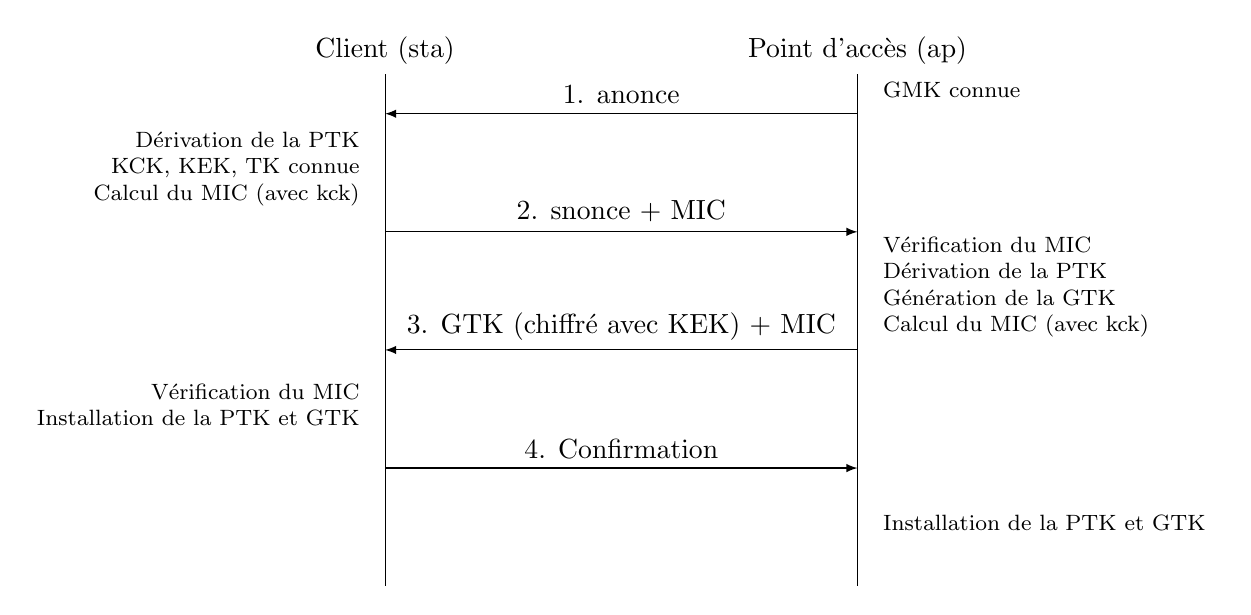
\begin{tikzpicture}[>=latex]

    \node (sta) at (0,0) {Client (\acrshort{sta})};
    \node (ap)  at (6,0) {Point d'accès (\acrshort{ap})};

    % Lignes de vie
    \draw (sta.south) -- ++(0,-6.5);
    \draw (ap.south)  -- ++(0,-6.5);

    % Messages
    \draw[->] (ap.south)++(0,-0.5) -- node[above,sloped]{1. \Gls{anonce}} ++(-6,0);
    \draw[->] (sta.south)++(0,-2) -- node[above,sloped]{2. \Gls{snonce} + MIC} ++(6,0);
    \draw[->] (ap.south)++(0,-3.5) -- node[above,sloped]{3. GTK (chiffré avec KEK) + MIC} ++(-6,0);
    \draw[->] (sta.south)++(0,-5) -- node[above,sloped]{4. Confirmation} ++(6,0);

    % Étapes locales STA (à gauche)
    \node[anchor=east, align=right, font=\footnotesize] 
    at (-0.2,-1.5) {%
    Dérivation de la PTK\\
    KCK, KEK, TK connue\\
    Calcul du MIC (avec \acrshort{kck})
    };

    \node[anchor=east, align=right, font=\footnotesize] 
    at (-0.2,-4.5) {%
    Vérification du MIC\\
    Installation de la PTK et GTK
    };

    % Étapes locales AP (à droite)
    \node[anchor=west, align=left, font=\footnotesize] 
    at (6.2,-0.5) {%
    GMK connue
    };

    \node[anchor=west, align=left, font=\footnotesize] 
    at (6.2,-3) {%
    Vérification du MIC\\
    Dérivation de la PTK\\
    Génération de la GTK\\
    Calcul du MIC (avec \acrshort{kck})
    };

    \node[anchor=west, align=left, font=\footnotesize] 
    at (6.2,-6.0) {%
    Installation de la PTK et GTK
    };

    \end{tikzpicture}
    \caption{4-Way Handshake WPA/WPA2}
    \label{fig:4way}
    \end{figure}

    La \textit{Pairwise Transient Key} (PTK) est en pratique un trousseau de sous-clés spécialisées : la KCK est utilisée pour l’authentification et la protection des messages du 4-Way Handshake, la KEK pour chiffrer et distribuer la clé de groupe GTK, et la TK pour chiffrer le trafic de données unicast entre la STA et le point d’accès.

    \begin{figure}[H]
        \centering
        \begin{tikzpicture}[
            box/.style={draw, rounded corners, minimum width=2.4cm, minimum height=0.9cm, align=center},
            smallbox/.style={draw, rounded corners, minimum width=2.2cm, minimum height=0.8cm, align=center, font=\footnotesize}
        ]

        \node[box] (ptk) {PTK\\(512 bits)};

        \node[smallbox, below=1.2cm of ptk] (kek) {\acrfull{kek}\\128 bits};
        \node[smallbox, left=0.2cm of kek] (kck) {\acrfull{kck}\\128 bits};
        \node[smallbox, right=0.2cm of kek] (tk) {\acrlong{tk}\\256 bits};

        \draw[->] (ptk) -- (kck);
        \draw[->] (ptk) -- (kek);
        \draw[->] (ptk) -- (tk);
        \end{tikzpicture}
        \caption{Décomposition de la PTK en sous-clés KCK, KEK et TK.}
        \label{fig:ptk-subkeys}
    \end{figure}

    Durant le 4-Way \Gls{handshake}, les messages ne sont pas chiffrés. Leur sécurité repose sur l’utilisation de la clé \acrshort{kck}, dérivée de la \acrshort{ptk}, permettant le calcul d’un \acrshort{mic} garantissant l’intégrité et l’authenticité des échanges. La clé \acrshort{kek} est quant à elle utilisée pour chiffrer la clé de groupe \acrshort{gtk} transmise par le point d’accès.

    \begin{table}[H]
        \centering
        \begin{tabular}{|l|l|l|l|l|l|}
        \hline
        \textbf{Clé} &
        \textbf{Taille} &
        \textbf{Usage} &
        \textbf{Phase} &
        \textbf{Renouvellement} \\
        \hline
        PSK &
        Variable &
        \Gls{passphrase} partagée &
        Pré-Phase &
        Manuel \\

        PMK &
        256 bits &
        Clé maître dérivée (PBKDF2) &
        Phase 1 &
        Ne change pas si PSK identique \\

        PTK &
        512 bits &
        Clé transitoire unicast &
        Phase 2 &
        À chaque 4-Way Handshake \\

        KCK &
        128 bits &
        Intégrité du handshake (MIC) &
        Phase 2 &
        À chaque 4-Way Handshake \\

        KEK &
        128 bits &
        Chiffrement de la GTK &
        Phase 2 &
        À chaque 4-Way Handshake \\

        TK &
        256 bits &
        Chiffrement des données unicast &
        Phase 3 & Clé par paquet (via TSC) \\

        GTK &
        128 bits &
        Trafic broadcast/multicast &
        Phase 2 &
        Périodique / Reconnexion \\
        \hline
        \end{tabular}
        \caption{Récapitulatif des clés utilisées dans WPA-TKIP}
        \label{tab:wpa_keys}
    \end{table}

    \item \textbf{Phase 3 (TKIP par trame)} : une fois la \acrshort{ptk} et la \acrshort{gtk} installées, WPA chiffre les données utilisateur à l’aide de l’algorithme \acrshort{tkip}.  
Contrairement à WEP, WPA garantit qu’une \textbf{clé de chiffrement distincte est utilisée pour chaque trame}, même si la clé maîtresse reste inchangée.

\medskip
Pour chaque trame transmise, TKIP s’appuie sur trois paramètres fondamentaux :
\begin{itemize}
    \item la \textbf{Temporal Key (TK)}, dérivée de la PTK ;
    \item l’\textbf{adresse MAC source}, liant cryptographiquement la trame à son émetteur ;
    \item le \acrfull{tsc}, un compteur de 48 bits.
\end{itemize}

\medskip
Le \acrshort{tsc} est incrémenté à chaque trame émise et joue un rôle central dans WPA-TKIP.  
Il assure à la fois :
\begin{itemize}
    \item l’\textbf{unicité de la clé de chiffrement par paquet} ;
    \item un \textbf{mécanisme anti-rejeu}, toute trame reçue avec un TSC déjà observé étant rejetée.
\end{itemize}

\medskip

Dans WPA utilisant TKIP, le champ appelé \textbf{IV} ne correspond plus à un vecteur d’initialisation aléatoire comme en WEP.  
Il transporte en réalité une représentation structurée du \acrfull{tsc}, d’où le terme d’\textit{IV étendu}.

\paragraph{Composition de l'IV étendu (32 bits dans la trame) :}  
Le champ IV envoyé dans la trame est une version codée et partielle du TSC, combinée avec le KeyID et quelques bits de contrôle :

\begin{itemize}
    \item \textbf{IV16 (bits 0-15) :} Correspond aux 16 bits de poids faible du TSC. Ces bits changent à chaque trame et garantissent l’unicité de la clé RC4 pour cette trame.  
    \item \textbf{IV8 (bits 16-23) :} Contient les 8 bits suivants du TSC.  
    \item \textbf{KeyID (2 bits) :} Ce champ identifie quelle clé de chiffrement parmi les clés partagées par le point d’accès et le client doit être utilisée pour cette trame. Il permet au récepteur de savoir quelle clé appliquer pour déchiffrer le paquet.  
    \item \textbf{Ext. IV / Reserved (6 bits) :} Ce champ complète le TSC en incluant les bits de poids fort (pour former les 48 bits du compteur de séquence) et peut également contenir des indicateurs de fragmentation ou des bits réservés pour la compatibilité.
\end{itemize}

\medskip
Afin de produire une clé RC4 unique pour chaque trame, TKIP applique un \textbf{mélange de clés en deux phases} (\textit{Key Mixing}) :

\medskip
\noindent
\textbf{Key Mixing – Phase 1 :}  
La première phase combine :
\begin{itemize}
    \item la \textbf{Temporal Key (TK)} ;
    \item l’\textbf{adresse MAC source} ;
    \item les \textbf{32 bits de poids fort du TSC} (\( \text{TSC}[47:16] \)).
\end{itemize}

Cette étape produit une \textbf{clé intermédiaire} spécifique à la station émettrice et au flot de transmission. 

\medskip
\noindent
\textbf{Key Mixing – Phase 2 :}  
La seconde phase affine cette clé intermédiaire en intégrant :
\begin{itemize}
    \item les \textbf{16 bits de poids faible du TSC} (\( \text{TSC}[15:0] \)) ;
    \item des \textbf{bits de contrôle de l’IV}, notamment les bits \textit{ExtIV} et des bits destinés à éviter les IV faibles (nommées \textit{d}).
\end{itemize}

Cette phase produit la \textbf{clé finale par trame}, appelée \acrfull{ppk}, utilisée comme entrée de l’algorithme RC4.  
Ainsi, même deux trames consécutives émises par une même station ne partageront jamais la même clé de chiffrement.

\medskip
Avant le chiffrement, un \acrshort{mic} est calculé sur les données en clair à l’aide de l’algorithme \textbf{Michael}.  
Ce MIC protège la trame contre les modifications actives et est concaténé aux données avant le calcul de l’\acrshort{icv} (CRC-32).

\medskip
L’ensemble \textit{(données || MIC || ICV)} est finalement chiffré par un XOR avec le flot de clés généré par RC4, produisant la trame WPA-TKIP transmise.

\newpage

\begin{figure}[H]
    \centering
    \begin{tikzpicture}[
        box/.style={draw, rectangle, minimum width=2.8cm, minimum height=0.9cm, align=center},
        smallbox/.style={draw, rectangle, minimum width=2.4cm, minimum height=0.7cm, align=center, font=\footnotesize},
        key_mixing/.style={draw, rectangle, fill=orange!70, minimum width=3cm, minimum height=0.9cm, align=center},
        rc4/.style={draw, rectangle, fill=blue!60, minimum width=3cm, minimum height=0.9cm, align=center},
        xor/.style={draw, rectangle, fill=green!60, minimum width=3cm, minimum height=0.9cm, align=center},
        arrow/.style={->, thick}
    ]

    % ====== TOP INPUTS ======
    \node[box] (iv) {IV \\ (48 bits)};
    \node[box, right=1.2cm of iv] (ptk) {TK \\ (128 bits)};
    \node[box, right=1.2cm of ptk] (mac) {Sender MAC \\ Address (48 bits)};

    % ====== KEY MIXING ======
    \node[key_mixing, below=1.2cm of ptk] (mix1) {Step 1 Key Mixing};
    \node[key_mixing, below=0.8cm of mix1] (mix2) {Step 2 Key Mixing};

    \node[smallbox, below=0.8cm of mix2] (ppk) {PPK \\ (104 bits)};

    \node[smallbox, left=0cm of ppk] (iv16_1) {IV \\ (16 bits)};
    \node[smallbox, left=0cm of iv16_1] (dbyte) {\texttt{d} \\ special byte};
    \node[smallbox, left=0cm of dbyte] (iv16_2) {IV \\ (16 bits)};

    % ====== RC4 ======
    \node[rc4, below=1.0cm of ppk] (rc4) {RC4};
    \node[box, below=1.0cm of rc4] (keystream) {Keystream};

    % ====== XOR ======
    \node[xor, right=1.4cm of keystream] (xor) {XOR};

    % ====== ARROWS ======
    \draw[arrow] (iv) |- node[left]{32 bits} (mix1);
    \draw[arrow] (iv) -| node[left]{16 bits} (iv16_2);
    \draw[arrow] (iv) |- node[left]{16 bits} (mix2);

    \draw[arrow] (ptk) -- (mix1);
    \draw[arrow] (mac) |- (mix1);

    \draw[arrow] (mix1) -- (mix2);
    \draw[arrow] (mix2) -- (ppk);
    \draw[arrow] (ppk) -- (rc4);
    \draw[arrow] (iv16_1) |- (rc4);
    \draw[arrow] (iv16_2) |- (rc4);
    \draw[arrow] (dbyte) |- (rc4);
    \draw[arrow] (rc4) -- (keystream);

    \draw[arrow] (keystream) |- (xor);
    \end{tikzpicture}
        \caption{Création keystream WPA\cite{WeaknessesWPA:online}}
        \label{fig:wpa_tkip_frame_1}
\end{figure}

\begin{figure}[H]
    \centering
    \begin{tikzpicture}[
        box/.style={draw, rectangle, minimum width=2.8cm, minimum height=0.9cm, align=center},
        smallbox/.style={draw, rectangle, minimum width=2.4cm, minimum height=0.7cm, align=center, font=\footnotesize},
        algo/.style={draw, rectangle, fill=blue!60, minimum width=3cm, minimum height=0.9cm, align=center},
        xor/.style={draw, rectangle, fill=green!60, minimum width=3cm, minimum height=0.9cm, align=center},
        arrow/.style={->, thick}
    ]

    % ====== TOP INPUTS ======
    \node[box] (plaintext_msdu) {Plaintext MSDU};
    \node[algo, right=1.0cm of plaintext_msdu] (miccalc) {MIC = Michael \\ (TK, SA, DA, Plaintext)};

    % ====== PLAINTEXT PATH ======
    \node[box, below=1.0cm of plaintext_msdu] (plaintext_mpdu) {Plaintext MPDU \\ (Plaintext || MIC)};
    \node[algo, right=1.0cm of plaintext_mpdu] (crc) {ICV \\ CRC-32};

    \node[box, below=1.0cm of crc] (plaintext_mpdu_final) {Plaintext MPDU};
    \node[smallbox, right=0cm of plaintext_mpdu_final] (crcgen) {ICV\\( 4 octets)};

    % ====== XOR ======
    \node[xor, right=1.4cm of crcgen] (xor) {XOR};

    % ====== ARROWS ======
    \draw[arrow] (plaintext_msdu) -- (miccalc);
    \draw[arrow] (plaintext_msdu) -- (plaintext_mpdu);
    \draw[->] (miccalc) -- ++(0,-0.8) -| (plaintext_mpdu);
    \draw[arrow] (plaintext_mpdu) -- (crc);
    \draw[arrow] (plaintext_mpdu) |- (plaintext_mpdu_final);
    \draw[arrow] (crc) -| (crcgen);

    \draw[arrow] (crcgen) -- (xor);

    \end{tikzpicture}
        \caption{Gestion plaintext WPA\cite{WeaknessesWPA:online}}
        \label{fig:wpa_tkip_frame_2}
\end{figure}
\end{itemize}

\begin{figure}[H]
    \centering
    \begin{tikzpicture}[
        box/.style={draw, rectangle, minimum width=2.8cm, minimum height=0.9cm, align=center},
        smallbox/.style={draw, rectangle, minimum width=2.4cm, minimum height=0.7cm, align=center, font=\footnotesize},
        xor/.style={draw, rectangle, fill=green!60, minimum width=3cm, minimum height=0.9cm, align=center},
        packet/.style={draw, rectangle, fill=red!70, minimum width=2.2cm, minimum height=0.8cm, align=center},
        arrow/.style={->, thick}
    ]

    % ====== XOR ======
    \node[xor] (xor) {XOR};

    % ====== OUTPUT FRAME ======
    \node[box, below=1.2cm of xor] (macheader) {MAC Header};
    \node[box, right=0cm of macheader] (ivkey) {IV / KeyID};
    \node[packet, right=0cm of ivkey] (dataout) {MSDU};
    \node[packet, right=0cm of dataout] (micout) {MIC};
    \node[packet, right=0cm of micout] (icv) {ICV};
    \node[box, right=0cm of icv] (fcs) {FCS};

    % ====== ARROWS ======
    \draw[arrow] (xor) -| (dataout);
    \draw[arrow] (xor) -| (micout);
    \draw[arrow] (xor) -| (icv);

    \end{tikzpicture}
    \caption{Paquet WPA final\cite{WeaknessesWPA:online}}
    \label{fig:wpa_tkip_full}
\end{figure}

% WPA2

\subsubsection{WPA2 : AES-CCMP et le 4-Way Handshake}

WPA2 apporte une amélioration profonde : l’abandon de RC4 au profit d’un chiffrement moderne AES-CCMP.

\subsubsection*{Modes d’authentification}
\begin{itemize}
    \item \textbf{WPA2-PSK} : la PMK (\textit{Pairwise Master Key} : clé maitresse) = PBKDF2(\textit{Password-Based Key Derivation Function 2} : basée sur une \gls{passphrase} et le SSID).
    \item \textbf{WPA2-Enterprise} : PMK fournie via un serveur RADIUS et une authentification EAP.
\end{itemize}

% WPA3 / SAE

\subsubsection{WPA3 : SAE, Dragonfly, GCMP et PMF}

WPA3 corrige des failles structurelles de WPA2, notamment KRACK, en introduisant SAE (Authenfication mutuelle des \acrshort{ap} et de la \acrshort{sta}) et le support obligatoire de l'algorithme de chiffrement GCMP.

% SAE / GCMP crypto details

\subsection{Mécanismes cryptographiques avancés}

Les protocoles de sécurité modernes du Wi-Fi reposent sur des mécanismes cryptographiques plus élaborés que ceux utilisés par les générations précédentes. Contrairement à WEP et TKIP, qui n’offraient qu’une protection minimale contre l’écoute, l’injection ou la manipulation des trames, WPA2 et surtout WPA3 reposent sur des constructions cryptographiques complètes, conçues pour fournir à la fois confidentialité, intégrité, résistance aux attaques par rejeu et garanties formelles sur la sécurité de la session.\\

Trois mécanismes occupent une place centrale : AES-CCMP, GCMP et SAE (aussi appelé Dragonfly). Ces protocoles ne jouent pas le même rôle, mais constituent ensemble la base de la sécurité Wi-Fi contemporaine.

\subsubsection{AES-CCMP}

AES-CCMP est devenu la norme de chiffrement par défaut avec WPA2. Son objectif est d’aller bien au-delà du simple masquage des données transportées : il assure simultanément la confidentialité des informations, l’intégrité des trames et la protection contre les attaques par rejeu.

Pour y parvenir, CCMP combine deux éléments complémentaires. D’une part, il utilise AES en mode compteur (CTR) pour le chiffrement. Ce mode transforme le bloc AES en générateur de flot chiffrant, permettant de chiffrer efficacement des paquets de taille variable sans introduire de structure exploitable. De l’autre, CCMP associe ce chiffrement à un code d’authentification basé sur CBC-MAC, un mécanisme cryptographique destiné à garantir que les données n’ont subi aucune altération.\\

Cette combinaison forme une construction dite \textit{AEAD} (Authenticated Encryption with Associated Data), dans laquelle confidentialité et intégrité sont assurées simultanément par une même clé, ce qui évite un grand nombre de vulnérabilités présentes dans les générations antérieures.

L’ensemble repose également sur un numéro de paquet (Packet Number, PN) utilisé comme nonce unique. Toute réutilisation est interdite, ce qui empêche un attaquant de rejouer ou de réinjecter des trames chiffrées. En pratique, AES-CCMP constitue encore aujourd’hui une référence en matière de chiffrement pour les réseaux Wi-Fi.

AES-CCMP combine :
\begin{itemize}
    \item AES en mode CTR pour le chiffrement ;
    \item CBC-MAC pour l'intégrité.
\end{itemize}

\subsubsection{GCMP (AES-GCM)}

GCMP, introduit avec les standards 802.11ac et repris dans WPA3-Enterprise, reprend les principes d’AES-CCMP mais s’appuie cette fois sur AES-GCM. Cette construction fait partie des modes de chiffrement AEAD les plus robustes. AES-GCM associe un chiffrement en mode CTR à la fonction d’authentification GHASH. Cette approche permet de calculer l’intégrité et le chiffrement de façon quasi parallèle, ce qui rend GCMP particulièrement performant sur les architectures modernes.\\

L’intérêt principal de GCMP réside donc dans sa rapidité : il offre un débit supérieur à CCMP, ce qui le rend bien adapté aux environnements à forte charge ou aux réseaux professionnels nécessitant des débits élevés.

\subsubsection{SAE / Dragonfly}

Contrairement à AES-CCMP et à GCMP, qui sont des mécanismes de chiffrement et d’intégrité utilisés \emph{après} l’établissement de la connexion, SAE (Simultaneous Authentication of Equals) intervient au moment de l’authentification. SAE n’est pas un algorithme de chiffrement mais un protocole d’échange de clés sécurisé.

L’enjeu de SAE est de résoudre l’un des problèmes fondamentaux des versions antérieures : avec WPA2-PSK, un attaquant pouvait capturer un 4-Way Handshake puis tenter hors ligne de retrouver le mot de passe par dictionnaire. Dans SAE, ce type d’attaque est impossible. Le protocole s'appuie sur un échange Diffie–Hellman, dans lequel le mot de passe n'est jamais transmis ni dérivé sous forme exploitable. Chaque tentative d’authentification nécessite une interaction en temps réel avec le point d’accès, ce qui empêche les attaques hors ligne et limite naturellement la vitesse des tests possibles.\\

SAE offre également la propriété de \textit{Forward Secrecy} : même si un mot de passe venait à être compromis ultérieurement, les sessions passées resteraient inexploitables, car la clé de session résulte d’un secret éphémère renouvelé à chaque connexion. Cette approche corrige l’une des failles les plus importantes de WPA2 et constitue la principale amélioration de WPA3-Personal.

Pour résumer, ses caractériques principales sont les suivantes :

\begin{itemize}
    \item s’appuie sur Diffie-Hellman ;
    \item offre Forward Secrecy ;
    \item empêche les attaques hors-ligne ;
    \item protège contre attaques dictionnaires massives.
\end{itemize}

% Synthesis table

\subsection{Synthèse comparative approfondie}

\begin{table}[H]
\centering
\begin{tabular}{|c|c|c|c|c|}
\hline
\textbf{Protocole} & \textbf{Crypto} & \textbf{Auth} & \textbf{Intégrité} & \textbf{Résistance} \\
\hline
WEP & RC4 & Clé statique & CRC-32 & Nulle \\
WPA & RC4 & PSK & MIC & Faible \\
WPA2 & AES-CCMP & PSK/802.1X & CBC-MAC & Forte (hors KRACK) \\
WPA3 & GCMP & SAE/802.1X & PMF & Très forte \\
\hline
\end{tabular}
\caption{Comparaison des protocoles de sécurité Wi-Fi}
\end{table}

\newpage